\chapter{Smart Contract Development}

In this Appendix we go over the steps a developer needs to go through in order to be able to code, test, debug and deploy DApps in Ethereum. 

\section{Setting up a development environment}
In this section we explain the installation steps for the software needed for DApp development. Basic Linux knowledge is assumed. The described steps are tested in Ubuntu 17.04.

Firstly, an Ethereum client implementation must be installed on the system. We choose geth\footnote{\url{https://github.com/ethereum/go-ethereum}}. We can download the latest version of geth from \url{https://github.com/ethereum/go-ethereum/releases}. 

\begin{lstlisting}[language=bash,caption={Installing geth}]
wget https://gethstore.blob.core.windows.net/builds/geth-linux-amd64-1.8.6-12683fec.tar.gzI
tar -zvf geth-linux-amd64-1.8.6-12683fec.tar.gz
mkdir ~/.local/bin
mv geth-linux-amd64-1.8.6-12683fec.tar.gz ~/.local/bin/geth
geth version
\end{lstlisting}

The tools that we will be using require NodeJS and Git. We install NodeJS via the Node Version Manager\footnote{\url{https://github.com/creationix/nvm}} in order to have better management over the NodeJS versions.

\begin{lstlisting}[language=bash,caption={Installing node and git }]
sudo apt install git
curl -o- https://raw.githubusercontent.com/creationix/nvm/v0.33.11/install.sh | bash
nvm install node
nvm alias default node
node --version
npm --version
\end{lstlisting}

We then install the tools and libraries used for having a proper development workflow. These tools are the Truffle Development Framework, Solium which is a linter to identify and fix style issues in Solidity, Web3.js which is the javascript library for interacting with the Ethereum ecosystem

\begin{lstlisting}[language=bash,caption={Installing development tools}]
npm install -g web3
npm install -g truffle
npm install -g solium
\end{lstlisting}

Finally, we install Ganache which provides us with the ability to launch local testnet instances with prefunded accounts for local testing. Ganache has both a Graphical User Interface and a Command Line Interface version.

\begin{lstlisting}[language=bash,caption={Installing ganache}]
npm install -g ganache-cli # command Line
wget https://github.com/trufflesuite/ganache/releases/download/v1.1.0/ganache-1.1.0-x86_64.AppImage 
mv ganache-1.1.0-x86_64.AppImage ~/.local/bin/ganache
chmod a+x ~/.local/bin/ganache # graphical interface
\end{lstlisting}

\begin{figure}[htb]
    \centering
    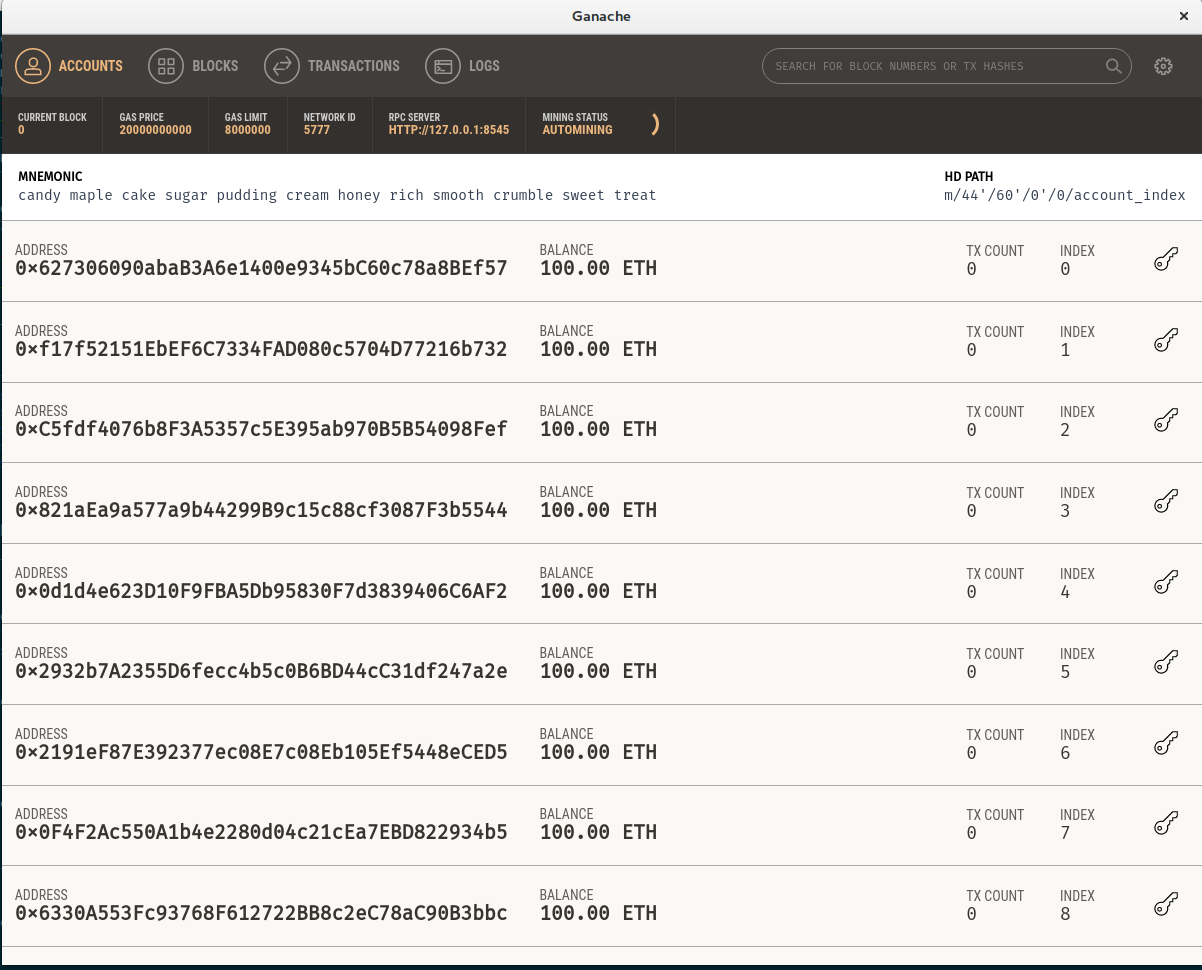
\includegraphics[width=1.0\textwidth]{ganache}
    \caption{Ganache User Interface}
    \label{fig:ganache}
\end{figure}

\section{Interacting with Ethereum}

By default, ganache starts listening at \texttt{localhost:8545} for incoming Ethereum JSON-RPC formatted messages\footnote{\url{https://github.com/ethereum/wiki/wiki/JSON-RPC}}, and has 10 pre-funded accounts with 100 ether, as shown in Figure \ref{fig:ganache}. In addition, any transaction that gets submitted gets instantly confirmed which allows for rapid debugging. We can attach to that and instance and interact with the testnet by using the command \texttt{geth attach http://localhost:8545}. 

After being connected to a new testnet instance we can query the node for the balances of each account as well as make transactions as shown in Figure \ref{fig:demo}.

\begin{figure}[htb]
    \centering
    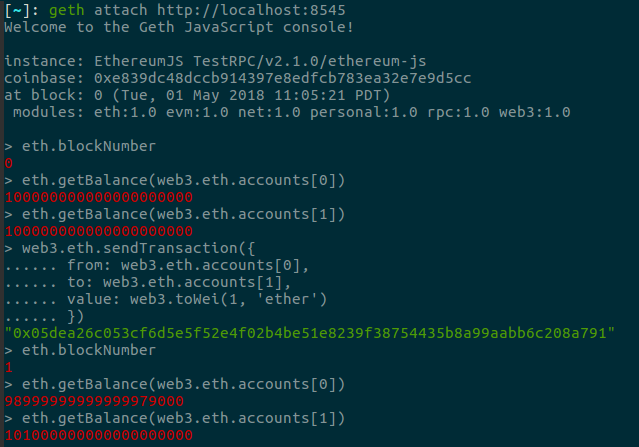
\includegraphics[width=0.8\textwidth]{transaction_demo}
    \caption{Querying a node and sending a transaction}
    \label{fig:demo}
\end{figure}

After a transaction gets submitted, its transaction hash is returned, and when it is mined in a block, its transaction receipt can be retrieved which contains additional information about that transaction as shown in \ref{fig:transaction}. Similarly, thet contents of a block can get fetched by querying \texttt{eth.getBlock(<number>)}.

\begin{figure}[htb]
    \centering
    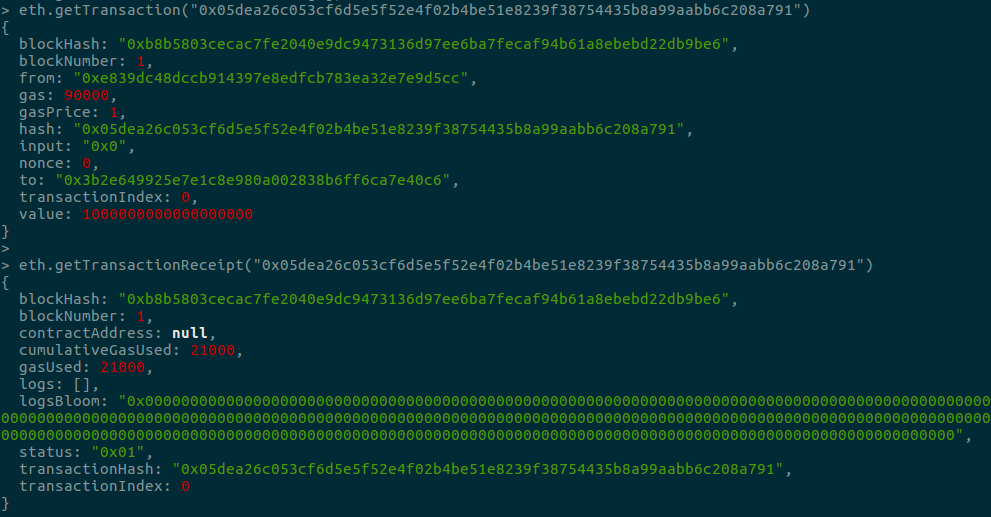
\includegraphics[width=1.0\textwidth]{tx-receipt}
    \caption{Contents of an Ethereum transaction when querying a node}
    \label{fig:transaction}
\end{figure}

\section{Development Workflow}

Truffle Framework and Ganache are the main tools used for smart contract development. When starting a new project, running the \texttt{truffle init} command results in the directory structure from Figure \ref{fig:truffle}. Developed smart contracts are placed under the directory \texttt{contracts}, the deployment scripts under \texttt{migrations} and finally Mocha\footnote{\url{https://mochajs.org/}} tests under \texttt{test}.

\begin{figure}[htb]
    \centering
    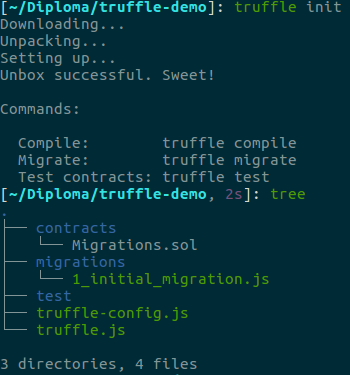
\includegraphics[width=0.4\textwidth]{truffle-demo}
    \caption{Directory structure after initializing a Truffle project}
    \label{fig:truffle}
\end{figure}

% TODO? Explain migrations with truffle migrate and testing with truffle test.

\section{Tool Development}

Having understood how \texttt{geth} is used for interacting with Ethereum and Truffle for developing, deploying and testing smart contracts, eventually we need to create our own tools. Web3 is the official library for interacting with Ethereum. We have already installed it for javascript, however we also use the python version for scripting client side and because we were more comfortable with tools written in Python. Web3.py is installed through pip with \texttt{pip install web3}. 

In case we want to interact with a public Ethereum network, we can either host our own local node and connect to \texttt{localhost:8545} like with ganache, or we can use a third-party public full node. Currently, the most reputable free provider for this service Infura\footnote{\url{https://infura.io/}}. Using Infura nodes requires first obtaining an API key. After that, interacting with a node is a matter if initializing the web3 instance, as shown in Figure \ref{fig:web3js} for Javascript and in Figure \ref{fig:web3py} for Python.

\begin{figure}[htb]
    \centering
    \lstinputlisting{code/web3.js}
    \caption{Interacting with a node in Javascript}
    \label{fig:web3js}
\end{figure}

\begin{figure}[htb]
    \centering
    \lstinputlisting{code/web3.py}
    \caption{Interacting with a node in Python}
    \label{fig:web3py}
\end{figure}